\chapter{X-ray Polarization Prospects for Blazars}
\label{chap:prospects}

\section{Introduction}

Polarization can be an important tool for probing the physics of the acceleration zone, especially in characterizing the magnetic field structures that control the expected shocks and induce synchrotron radiation. VLBI polarization maps have long been effective at measuring jet fields at pc-scale (e.g., \citealp{hovatta_mojave_2012}) while more recently optical polarization has provided new information on the field orientation and variability in the unresolved core \citep{blinov_robopol:_2018}. X-ray polarization, to be measured by the approved  Imaging X-ray Polarimetry Explorer ({\it IXPE}, \citealp{weisskopf_overview_2018}, launch 2021) and Enhanced X-ray Timing and Polarization mission ({\it eXTP}, \citealp{zhang_extp_2017}, launch $\sim$2025), offers new opportunities to probe the jet fields and radiation physics, even closer to the acceleration site. In particular, polarization can help answer whether leptonic or hadronic process dominate in a given band (e.g., \citealp{zhang_polarization_2016}).

However, the sensitivities of the near-future missions are modest and long exposures will
be required, so in light of the variability and limited low energy polarization information one
must choose the expected targets with care. We explore such choice here based on a simple synchro-Compton model. In section \ref{sec:xray_var} we characterize the X-ray variability of sources observed in optical polarization monitoring programs, in section \ref{sec:xray_predict} we use our model to predict X-ray polarization levels ($\rm\Pi_X$), while in section \ref{sec:xray_detect} we combine these factors to quantify the success probability of an {\it IXPE} measurement for reasonable exposure in an untriggered observation, identifying a list of prime targets, and suggesting other X-ray bright sources that can also be of interest if they exhibit strong optical polarization. We conclude by discussing new measurements that can improve these predictions and monitoring campaigns that could make additional sources, and additional classes of polarization behavior, accessible in the X-ray band.

\section{Detecting X-ray polarization in blazar jets}

\subsection{X-ray variability}
\label{sec:xray_var}

\begin{figure}
\resizebox{\hsize}{!}{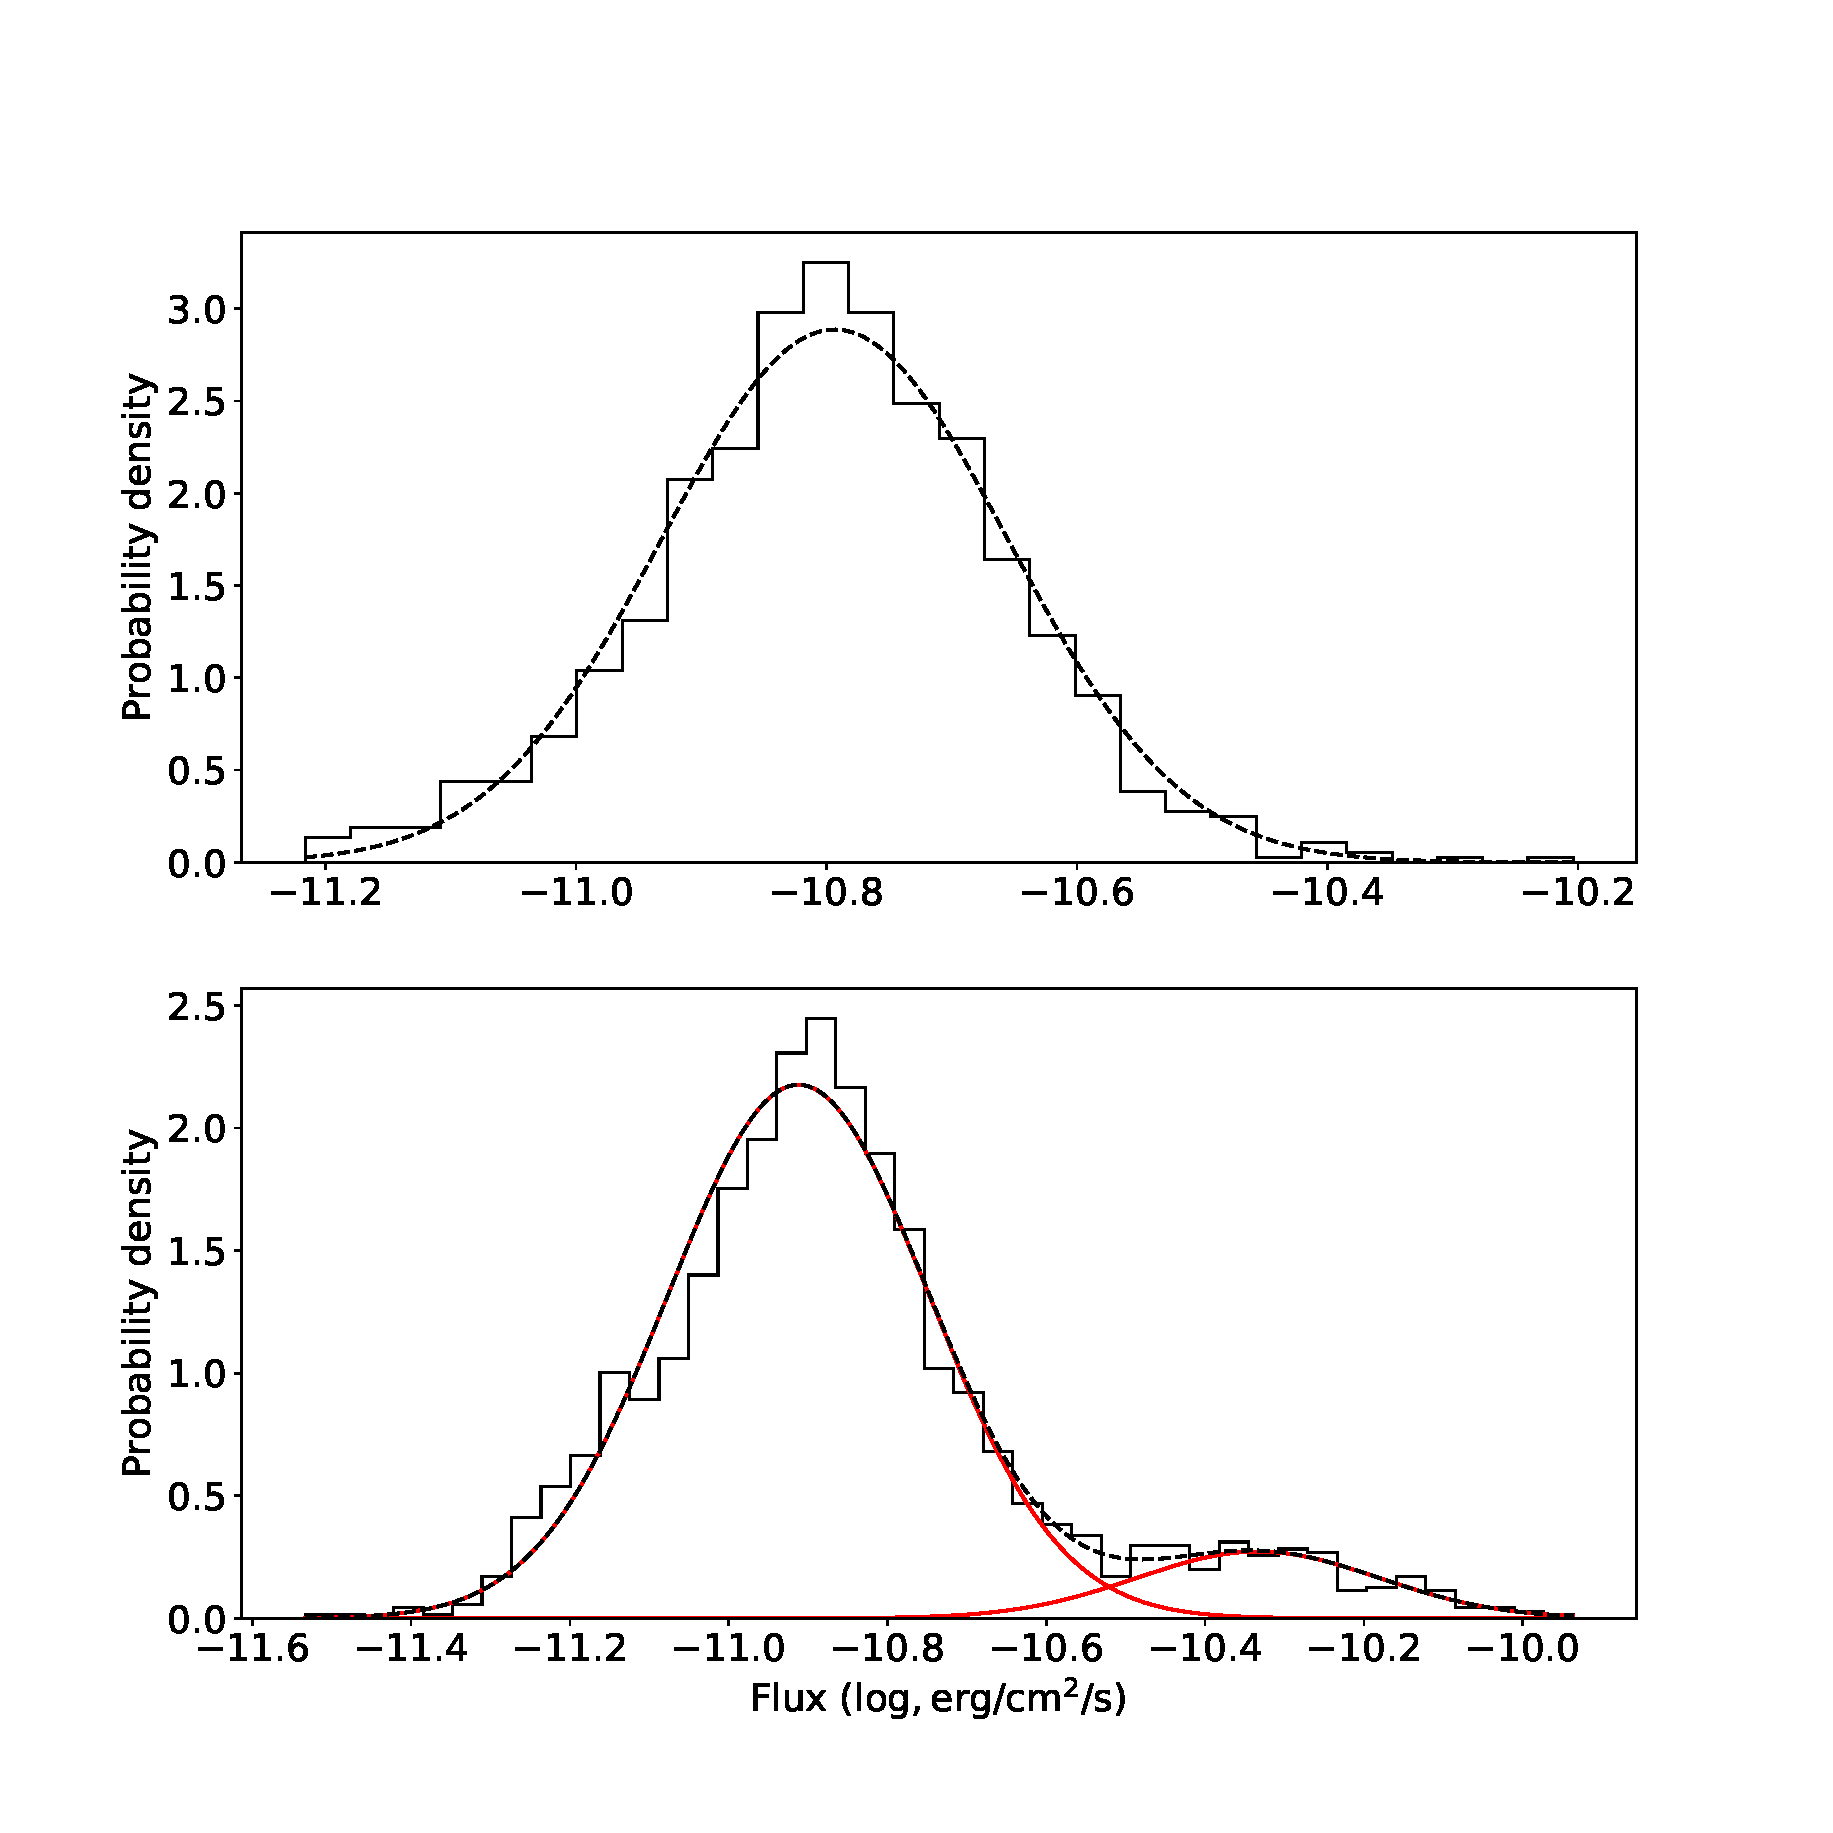
\includegraphics[scale=1]{example.eps} }
\centering
\caption{Example of a unimodal (top panel) and a bimodal (bottom panel) flux distribution in 
the 2-10~keV energy range in log-space. The black dashed line shows the best-fit model. In the bimodal case, 
the red lines show the individual components.}
\label{fig:example_hist}
\end{figure}

Since X-ray polarization measurements are in general sensitivity limited, source flux variability
plays a key role in the prospects for a secure, 99\% confidence, measurements of a given expected
polarization level. We must therefore characterize the variability of likely targets, the great
majority of which turn out to be sources detected by the {\it Fermi} LAT \citep{acero_fermi_2015}. 
We use 2-10\,keV flux measurements from 2005-2017 measured by the
Neil Gehrels {\it Swift} Observatory's (hereafter {\it Swift}) LAT source monitoring 
program\footnote{https://www.swift.psu.edu/monitoring/} \citep{strohmayer_statistical_2013} supplemented by 
2-10~keV fluxes (from 1995-2012) from the RXTE AGN timing and spectral 
database\footnote{We have included all sources in the RXTE database
classified as either BL Lac object (BL Lac) or Flat Spectrum Radio Quasar (FSRQ) with at least 20 observations. https://cass.ucsd.edu/$\sim$rxteagn/} \citep{rivers_full_2013}. 
\citet{strohmayer_statistical_2013} analyze the individual {\it Swift} observations; we employ their mean 
spectral parameters tabulated for each source to convert epoch count rates to $\rm erg/cm^2/s$ (2-10\,keV) using WebPIMMS. 35 sources (19 LSPs, 2 ISPs, 13 HSPs and one unclassified source\footnote{SED classification from the
3rd {\it Fermi} AGN catalog \cite{acero_fermi_2015}, https://www.ssdc.asi.it/fermi3lac/}) have at least
20 observations so that we can attempt a detailed variability analysis. For the remainder, we characterize
their flux variability with a simple mean and standard variation.

	Blazar high energy variability has been modeled as a log-normal distribution 
(e.g., \citealp{romoli_flux_2018,shah_log-normal_2018}), which may reflect disk-driven fluctuations \citep{lyubarskii_flicker_1997}
or variations in the jet particle acceleration \citep{sinha_flux_2018}. This suffices for some of our sources,
but others show wider variability. This may indicate multiple jet states (e.g. quiescent and active
flaring episodes), which can be represented by a double normal (Gaussian mixture) model (in log-space)
\citep{liodakis_bimodal_2017}. Of course if we have not sampled the full range of a source's variability the 
two log-normals might be subsets of a broader single log-normal. Here, using the historical fluxes,
we represent our flux distribution functions as either single or double log-normal models
without attaching physical significance to the single or double-mode behavior.

The likelihood function for the single Gaussian model is defined as
 \begin{eqnarray}
l_{\rm obs}&=&\frac{1}{\sqrt{2\pi(\sigma_{\rm q}^2+\sigma_{\rm obs}^2)}}
\exp\left[-\frac{(S_{\rm q}-S_{\rm obs})^2}{2(\sigma_{\rm q}^2+\sigma_{\rm obs}^2)}\right],
\end{eqnarray}
where $\rm S_{\rm q}$ and $\rm \sigma_{\rm q}$ are mean and standard deviation of the underlying distribution 
and $\rm S_{\rm obs}$ and $\rm \sigma_{\rm obs}$ are the observed fluxes and their uncertainties (in log-space). For the 
Gaussian mixture the likelihood is defined as
\begin{eqnarray}
l_{\rm obs}&=&\frac{1-f}{\sqrt{2\pi(\sigma_{\rm q}^2+\sigma_{\rm obs}^2)}}\exp\left[-\frac{(S_{\rm q}-S_{\rm obs})^2}{2(\sigma_{\rm q}^2+\sigma_{\rm obs}^2)}\right]\nonumber\\
&+&\frac{f}{\sqrt{2\pi(\sigma_{\rm a}^2+\sigma_{\rm obs}^2)}}\exp\left[-\frac{(S_{\rm a}-S_{\rm obs})^2}{2(\sigma_{\rm a}^2+\sigma_{\rm obs}^2)}\right].
\end{eqnarray}
where we add mean and standard deviation $\rm S_{\rm a}$ and $\rm \sigma_{\rm a}$ for a brighter `active' state
which is realized a fraction $\rm f$ of the observed samples. With such a model, we can draw an arbitrary number
of samples from the modeled distribution. To choose between models for a given source we use the Bayesian 
Information criterion (BIC).  Figure \ref{fig:example_hist} shows examples of best-fit models for 
PKS 0558-504 (top panel) and BL Lacertae (bottom panel). There are 15 sources best described as unimodal,
20 sources prefer a bimodal distribution. LSPs show no preference while HSPs slightly more
commonly match a bimodal distribution (8 versus 5).  The parameters of the best-fit distributions for 
all the sources are given in Table \ref{tab:par_sources}. For sources with $<20$ observations,
we simply record the mean and variance of the log of the flux, which can be used to form a log-normal distribution.

 Measurements are easiest for high polarization $\rm \Pi_X$ sources in bright large $\rm S_{\rm obs}$ states. 
Since both quantities are highly variable, we should test if they correlate, 
as might be expected from e.g. shock-driven flares (e.g., \citealp{marscher_core_2008}). Of course we lack $\rm \Pi_X$,
so we use the optical polarization ($\rm \Pi_O$) from the Robopol and Steward observatory monitoring programs which have significant
temporal overlap with the {\it Swift} data for 17 sources. We use optical polarization as a tracer of the energetic
electrons at the jet base that may also contribute X-ray synchrotron; radio
polarization can be dominated by downstream emission. While we cannot make meaningful statements about individual
sources, we can check the major source classes by stacking all contemporaneous observations from, say, the HSP.
We find that both the LSP and HSP have a mild positive correlation (Spearman's $\rm \rho\sim0.12$, significance $\rm p-value < 0.05$).
The two ISP showed no correlation. Thus for LSPs and HSPs we draw a flux at
a given level in their cumulative distribution function (CDF, e.g. a flux in the top X\%) and then draw from that source's polarization CDF at the same top X\% level. For the ISP we will assume random uncorrelated draws (see \S \ref{sec:duty_cycle}).
In practice, we find that this makes a small $<20$\% difference to the source detectability, so this assumption is not critical. However it should be tested with future monitoring campaigns.


\subsection{Expected X-ray polarization}
\label{sec:xray_predict}

	We must use the lower energy (optical) polarization degree $\rm \Pi_O$  to predict the polarization in
the X-ray band. For the HSP and some ISP, the X-rays come from the same (synchrotron) component,
while for the LSP and many ISP, they come from the low energy end of the high energy (here assumed
to be Compton) peak. Particularly interesting are the ISP for which the synchro-Compton transition
occurs within the {\it IXPE} band.
To quantify this connection we adopt a multizone jet picture, \cref{chap:synch},
where the observed modest $\rm \Pi_O$ are the result of incoherent averaging of $\rm N_{eff}$ effective emission 
zones, each of which radiates with the $\rm \Pi_{max} \approx 70\%$ expected for a uniform field, for a power-law
population of electrons with index $\approx 2$, producing the observed synchrotron spectrum. From observed polarization
levels we typically infer $\rm N_{eff} \approx 30-100$ for the emission cone contributing to the Earth line-of-sight.
In practice, the zones have different angles to the line-of-sight and different characteristic particle energies $\gamma_{max}$
so the number of zones, and thus $\rm \Pi$, becomes a function of the observation frequency 
(e.g. \citealp{marscher_rapid_2010, marscher_turbulent_2014}, and \cref{chap:ssc}. 

This multizone picture, with distributions in $\gamma_{max}$ and B field orientation, generally improves the match to observed blazar SEDs over that of a single-zone model. It also means that the $\rm \nu_{Sy}$ for the individual zones vary and so the number of zones $\rm N_{\rm eff}$ contributing half of the integrated flux is a function of
frequency. A computation with $\rm N_{\rm eff}$ related to the peak of the integrated spectrum, assuming typical
jet beaming parameters, $\rm B =0.1~G$ and a uniform squared distribution of $\gamma_{max}$ randomly distributed among
the zones is shown in the inset of Figure \ref{fig:Nzones}. The consequence is $\rm \Pi \approx \Pi_{max}/2\sqrt{N_{\rm eff}}$,
with a small increase from the incoherently averaged half of the flux from the remaining zones (see \cref{chap:ssc} for details). Thus 
$\rm N_{\rm eff}(\nu/\nu_{\rm peak})$ lets us relate the polarization at different frequencies across the
synchrotron component. Note that the $\rm N_{\rm eff}$ decrease and $\Pi$ increase can be dramatic for
$\nu \sim 10^3 \nu_{\rm peak}$; some ISPs can be in this regime.

The behavior in Figure \ref{fig:Nzones}, where the $\gamma_{max}$ range is more important than the effective
Doppler factor variation, is slightly conservative. In some models, such as the shock model of \citet{marscher_turbulent_2014},
$\gamma_{max}$ may depend on the angle of $B$ to a shock front and hence to the jet axis;
this organized variation further decreases $\rm N_{\rm eff}$ when one is well above the synchrotron
peak.  We find that this effect is only important for $3<\log(\nu/\nu_{peak})<4$, but there the polarization
increase can be as much as an additional $\sim 2\times$; a few ISPs may have synchrotron X-rays from this extreme regime.


\begin{figure}
\resizebox{\hsize}{!}{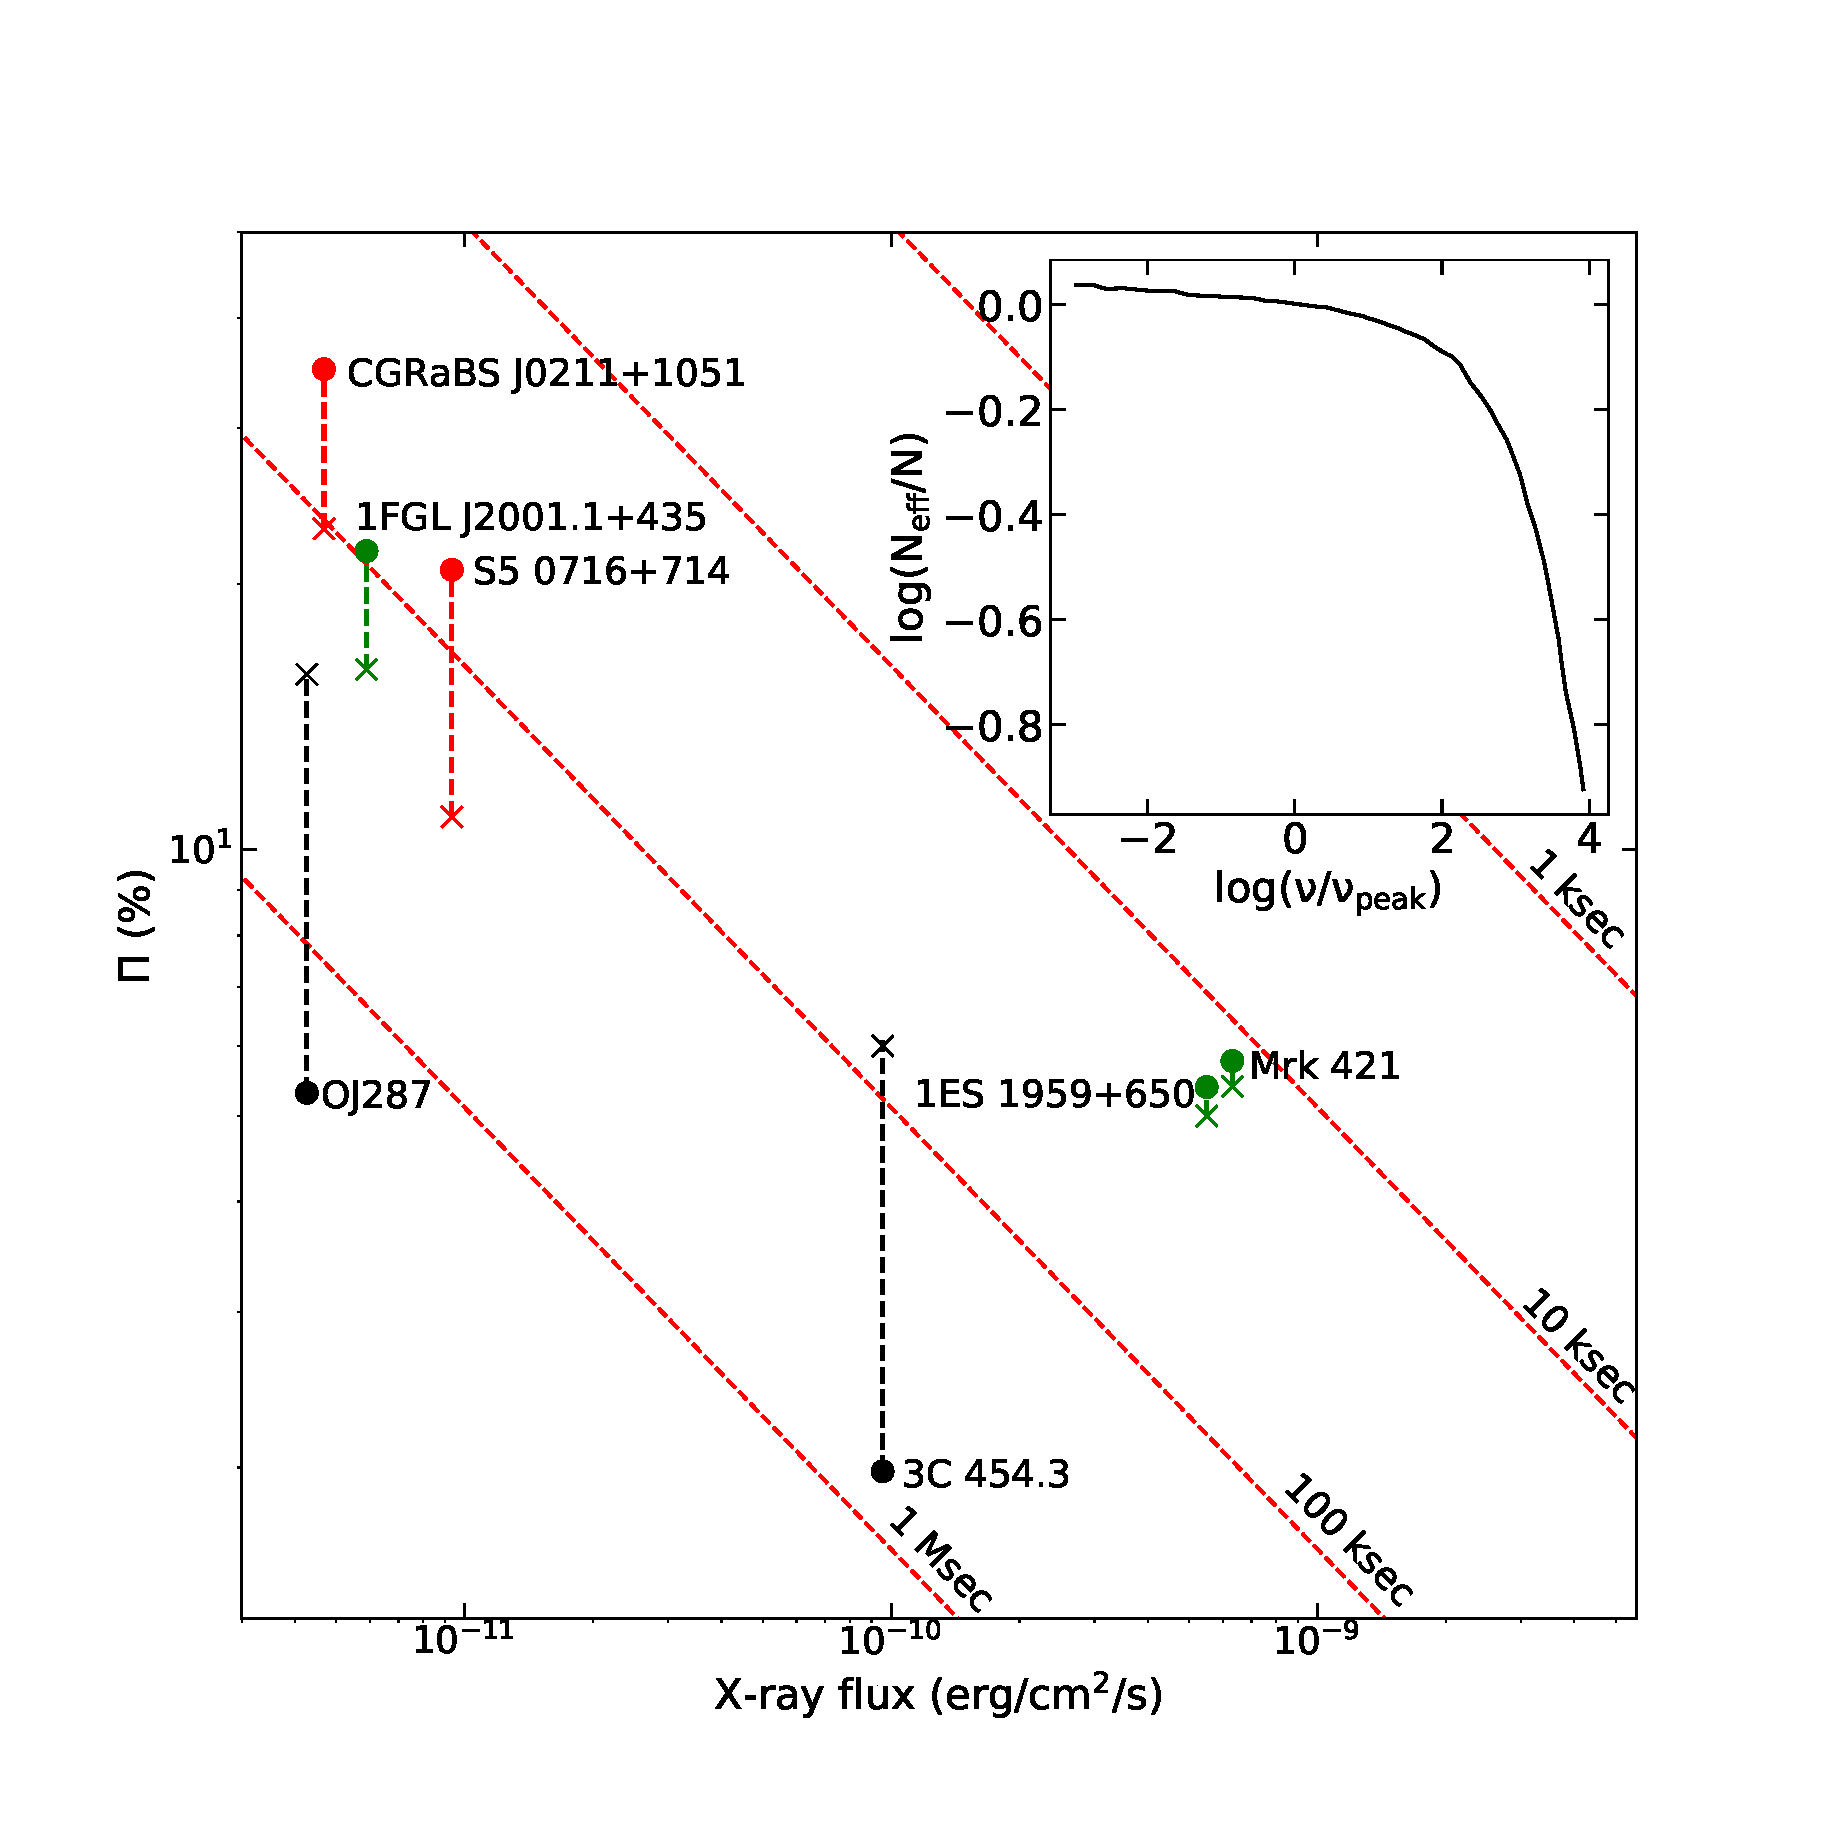
\includegraphics[scale=1]{multipanel.eps} }
\centering
\caption{The dashed lines show the shift from observed (optical, ``x'') to predicted (X-ray, ``dots'') $\rm \Pi$
for a few objects in each source class: LSP (black), ISP (red) and HSP (green). The diagonal lines show the {\it IXPE} sensitivity for a source with photon index $\approx2$ in a given exposure time.
Inset shows the frequency dependence of the effective zone number 
using the median Lorentz factor and viewing angle from \cite{liodakis_detecting_2017}.}
\label{fig:Nzones}
\end{figure}

For HSP we can directly convert the optical band polarization level to the X-ray band using the 
square root of the ratios of the $\rm N_{\rm eff}(\nu)$. We truncate at $\rm N_{eff}=1$ since our statistical 
estimate breaks down anyway. For some ISP, the $\rm \Pi$ increase can be substantial 
as long as the Compton component contributes weakly at 1-10\,keV. For ISPs, we used the Space Science Data 
Center (SSDC) tools\footnote{https://tools.ssdc.asi.it/SED/} to construct the SED of each source 
and determine whether the X-ray emission is synchrotron dominated. If so, we expect a substantial $\Pi$ increase compared to the optical. 

For LSP (and ISP with hard X-ray spectra) our model assumes that we observe Compton X-ray flux. This will only show polarization if the seed photon population is highly polarized (e.g., synchrotron emission). 
\cref{chap:ssc} find that for isotropic, many-zone scatting in typical jet geometries
the resulting Compton polarization is $0.2-0.36\times$ that of the seed photons. This
does depend on the viewing angle, opening angle, and Lorentz factor of the jet (see \cref{chap:ssc} for details).
However for the typical jet parameters assumed in the present work \citep{liodakis_detecting_2017} the retained polarization is near
maximal, so we will assume $\Pi_{\rm Comp} = 0.36 \times \Pi_{\rm seed}$. To get the latter, we scale from
$\rm \Pi_O$ using Fig. \ref{fig:Nzones}. For X-ray Compton emission typical seed photons are
in the mm-band, we will assume here $\sim 100$\,GHz, but the dependence on the weighted 
effective seed photon frequency is weak. Note that we are assuming that all seed photons are
synchrotron. If external photons contribute to the seed photon population $\Pi_{\rm Comp}$ will be lower.
This means that our estimates of the LSP polarization may be optimistic. This is useful
since any observed LSP polarization {\it higher} than our estimate indicates that the emission
should be non-Compton in nature (e.g., proton synchrotron).


	With these two effects we predict a $\rm \Pi_X$ for each source (Table \ref{tab:xpol_pred}).
Figure \ref{fig:Nzones} shows the shift from $\rm \Pi_O$ to $\rm \Pi_X$ for a few sources in each class, 
with an inset showing the $\rm N_{\rm eff}$ dependence on frequency.

\subsection{Blazar Detectability}
\label{sec:xray_detect}

\begin{figure}
\centering
\resizebox{\hsize}{!}{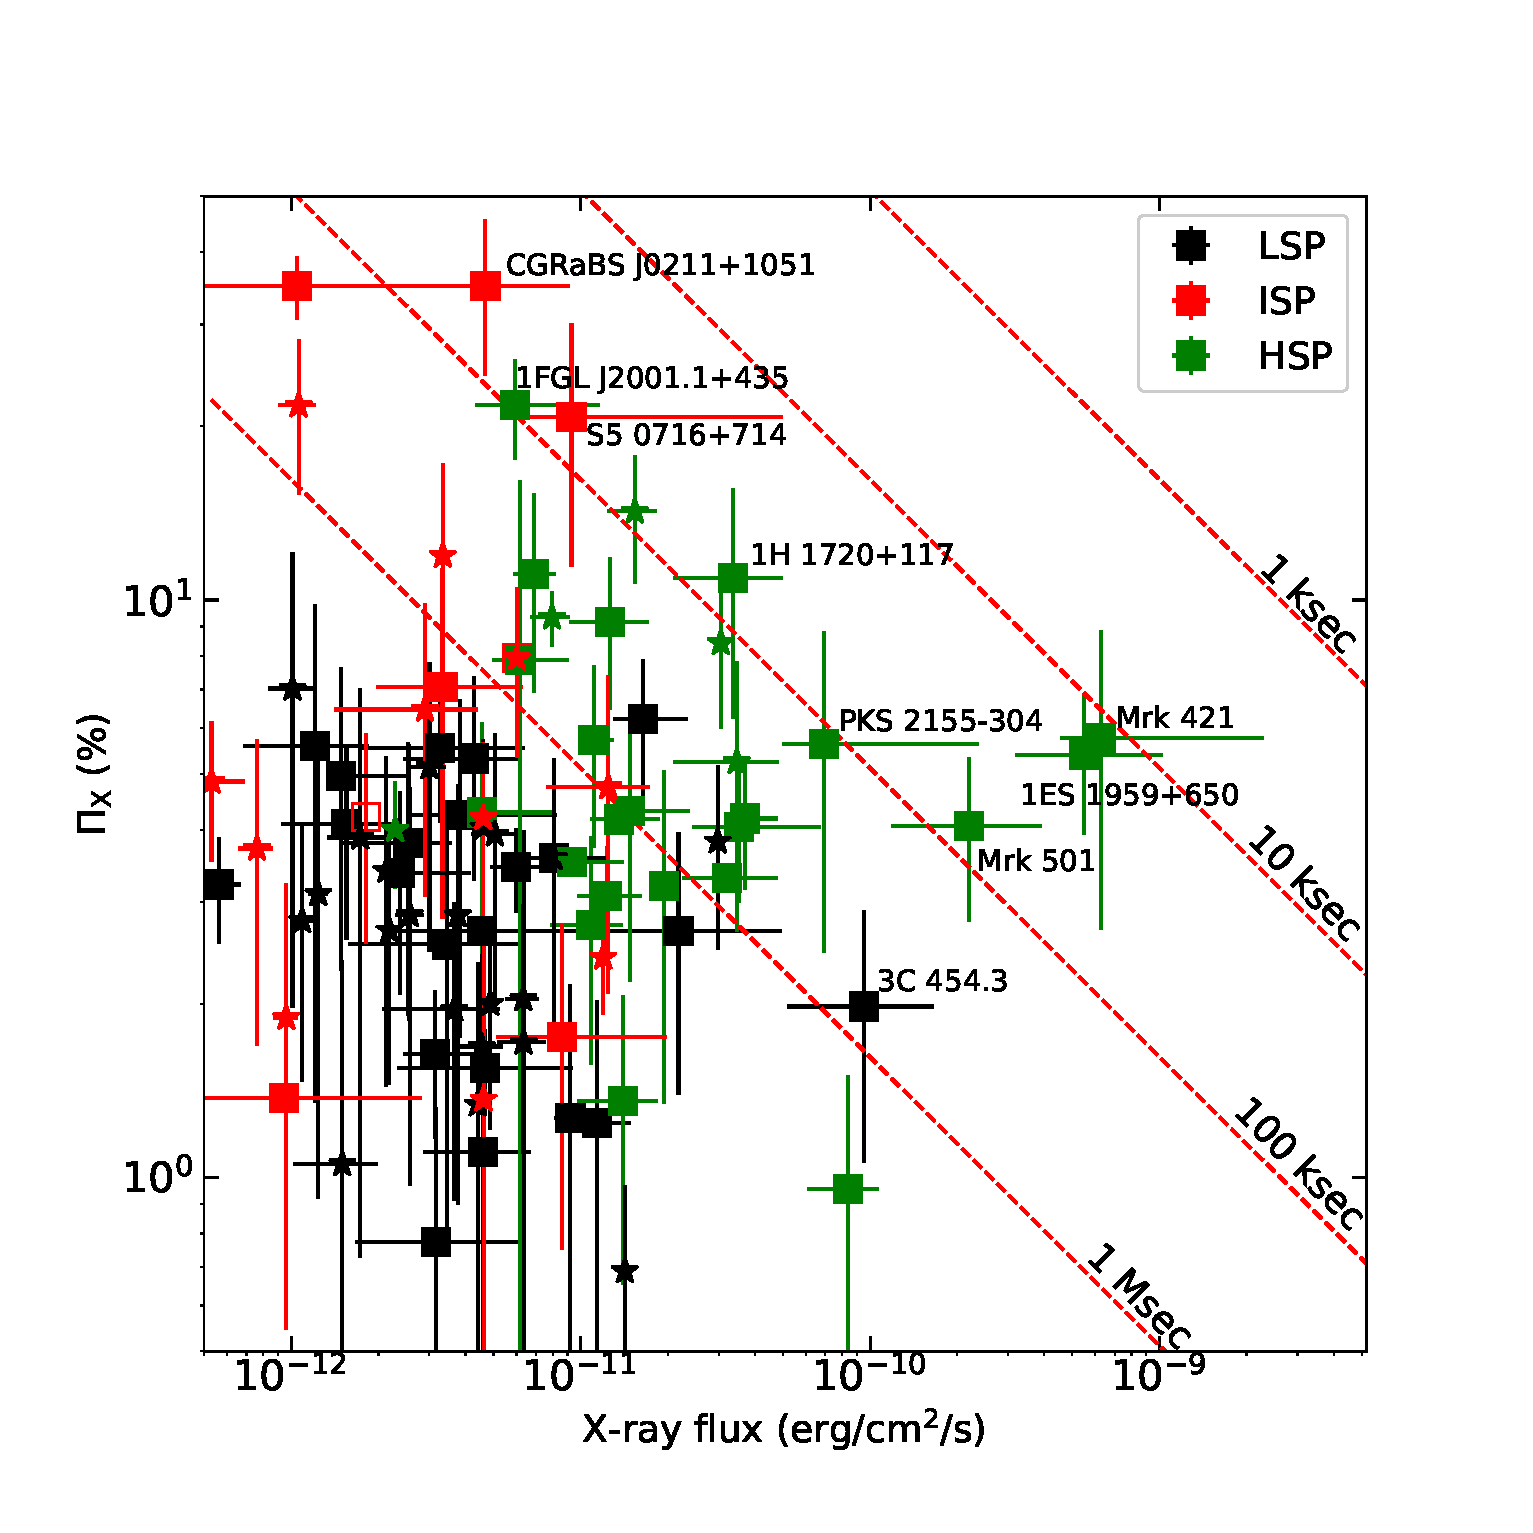
\includegraphics[scale=1]{prediction_IXPE_rescaled.eps} }
\caption{Predicted X-ray polarization degree versus the X-ray flux: LSP (black), ISP (red) and HSP (green).
Lines show the $\rm 1\sigma$ variability range in each quantity. Sources lacking at least 3 observations
each in $\rm S_X$ and $\rm \Pi_O$ are shown by open squares. Stars have $>3$ measurements in one quantity, solid
squares have $>3$ in both.  Red dashed lines show simple estimates for {\it IXPE} sensitivity for a source with photon index $\approx2$
in a given exposure time.}
\label{fig:pred_ixpe}
\end{figure}

Our prime target candidates are the sources measured with the RoboPol 
program\footnote{http://robopol.org/} \citep{pavlidou_robopol_2014,blinov_robopol:_2018} and the Steward 
observatory\footnote{http://james.as.arizona.edu/$\sim$psmith/Fermi/} \citep{smith_coordinated_2009}. 
For some of these we have {\it Swift} and/or RXTE monitoring, and so can construct a detailed
variability model (\S \ref{sec:xray_var}). For the remainder we collect typical fluxes from
the HEARSAC\footnote{https://heasarc.gsfc.nasa.gov/} database. There are 103 
sources with known SED class and at least one measurement in optical polarization and X-ray flux.

	Armed with estimates of the X-ray flux and polarization $\rm \Pi_X$ and their variability
we can make predictions for detectability. We focus on {\it IXPE} as the most imminent facility, whose
sensitivity is estimated using the dedicated online tools\footnote{https://ixpe.msfc.nasa.gov/cgi-aft/w3pimms/w3pimms.pl} \citep{soffitta_ixpe_2017,odell_imaging_2018}. Typical exposures will be $\sim 100\,$ksec, although the longest may approach a Msec. Figure 
\ref{fig:pred_ixpe} shows the X-ray flux and predicted X-ray polarization degree using the median 
and 1$\rm \sigma$ confidence intervals from the PDFs for each source. These PDFs are
estimated following \S\ref{sec:xray_predict}. Note that with our assumed 
correlated fluctuations, HSP and LSP will vary diagonally (UR to LL) within these error bands.
As expected, several HSPs are detectable at 100~ksec while a few (e.g., Mrk 421) might give
significant measurements in 10~ksec, allowing a detailed variability study. Only few LSP sources
are detectable, even with Msec exposures, under typical conditions.  A few 
(e.g., 3C~454.3) are occasionally accessible in shorter time when bright 
and highly polarized.


\subsubsection{Detectability Duty Cycle}
\label{sec:duty_cycle}

We must consider the substantial flux (\S \ref{sec:xray_var}) and polarization variability (e.g., \citealp{angelakis_robopol:_2016,kiehlmann_optical_2017}) when predicting the success of an X-ray polarization search. The uncertainty ranges in Figure \ref{fig:pred_ixpe} already give
some idea of these effects. But some sources vary well outside these ranges, especially
in occasional large $\rm S_X$ flares and less often in polarization increases. Thus we use
distribution function models to characterize the full variability range. For the X-ray variability we either use the parameters in Table \ref{tab:par_sources} to construct a flux distribution function or use the mean and standard deviation to define a single log-normal model (see \S \ref{sec:xray_var}). For the optical polarization, we use distribution 
functions from the maximum likelihood modeling results of \cite{angelakis_robopol:_2016} for RoboPol sources; for Steward Observatory-monitored sources we use their empirical CDF \citep{smith_coordinated_2009}. As noted above for the ISPs we draw randomly for the CDFs, while for LSPs and HSPs we draw an $\rm S_X$ and then adopt $\rm \Pi_X$ from the same probability level.  We consider only sources with at least three observations in both optical polarization and X-ray 
flux and estimate the joint detection probability (DP) by computing the $\rm MDP_{99}$ in a given exposure time and comparing with the predicted $\rm \Pi_X$. We consider
a simulated observation as a detection if $\rm \Pi_X > MDP_{99}$. By repeating this 
calculation $10^4$ times we estimate the fraction of trials a source was detected. 
Dropping the flux-$\Pi$ correlations results in $<20\%$ decrease in the LSP, HSP 
detectability estimates. For the RXTE and {\it Swift} monitored sources we use the average spectral parameters and WebPIMMS to estimate the $\rm MDP_{99}$ from the drawn flux value. For the remaining sources we use a photon index of 1.5 for inverse Compton and 2.5 for synchrotron emitting sources. In any case, assuming different spectral parameters results in only $\sim 5\%$ change in DP. Table \ref{tab:duty_cycle} gives these detection probability values for an assumed 100\,ksec {\it IXPE} exposure. They can be interpreted as the chance of success for a random observation at this exposure, or as the duty cycle for a triggered (by e.g., flux and/or $\rm \Pi_O$ monitoring) campaign. Of course, if one wants to measure a particular source, one can obtain more acceptable detection odds by increasing the exposure duration. While several HSPs have reasonable detection probabilities, only one ISP (CGRaBs~J0211+1051) and one LSP (3C~454.3) are detected at $>$10\% duty cycle. Thus long monitoring campaigns to allow bright trigger thresholds and/or longer {\it IXPE} exposures will be needed to reliably detect these source classes. It should be noted that source $\rm \Pi_O$ can vary by $2\times$ over a few days so longer exposures are not strictly `snapshots' as computed here. Intraday variability is seen, but is uncommon enough to leave our $\sim$1 day detectability estimates unaffected.

\subsubsection{Sources without measured optical polarization}

While many of the best and brightest candidates have been observed in existing optical
polarization campaigns, there are other blazars that might be of interest. For example we find
208 blazars from the BZ catalog \citep{massaro_5th_2015} present in the {\it Swift} master catalog,
97 of which have $S_X>5\times10^{-13}$ and a known spectral $\rm \nu_{Sy}$ class, so that
we can evaluate their observability as a function of the
unknown optical polarization level. With the observed X-ray flux we estimate 
the $\rm MDP_{99}$ (accounting for the different source spectra as in section \ref{sec:duty_cycle}) as a function of exposure time. We convert this to expected optical polarization 
using the relation in Fig. \ref{fig:Nzones}. Figure \ref{fig:nopol} and Table \ref{tab:no_pol} show 
the best prospects from this exercise. Table \ref{tab:no_pol} also lists the 
minimum optical polarization that we would require for $\sim$100\,ksec {\it IXPE} detections.
This suggests that several more HSP and a few ISP are accessible in reasonable 
exposures, although one should obtain reconnaissance $\rm \Pi_O$ measurements first.

\begin{figure}
\resizebox{\hsize}{!}{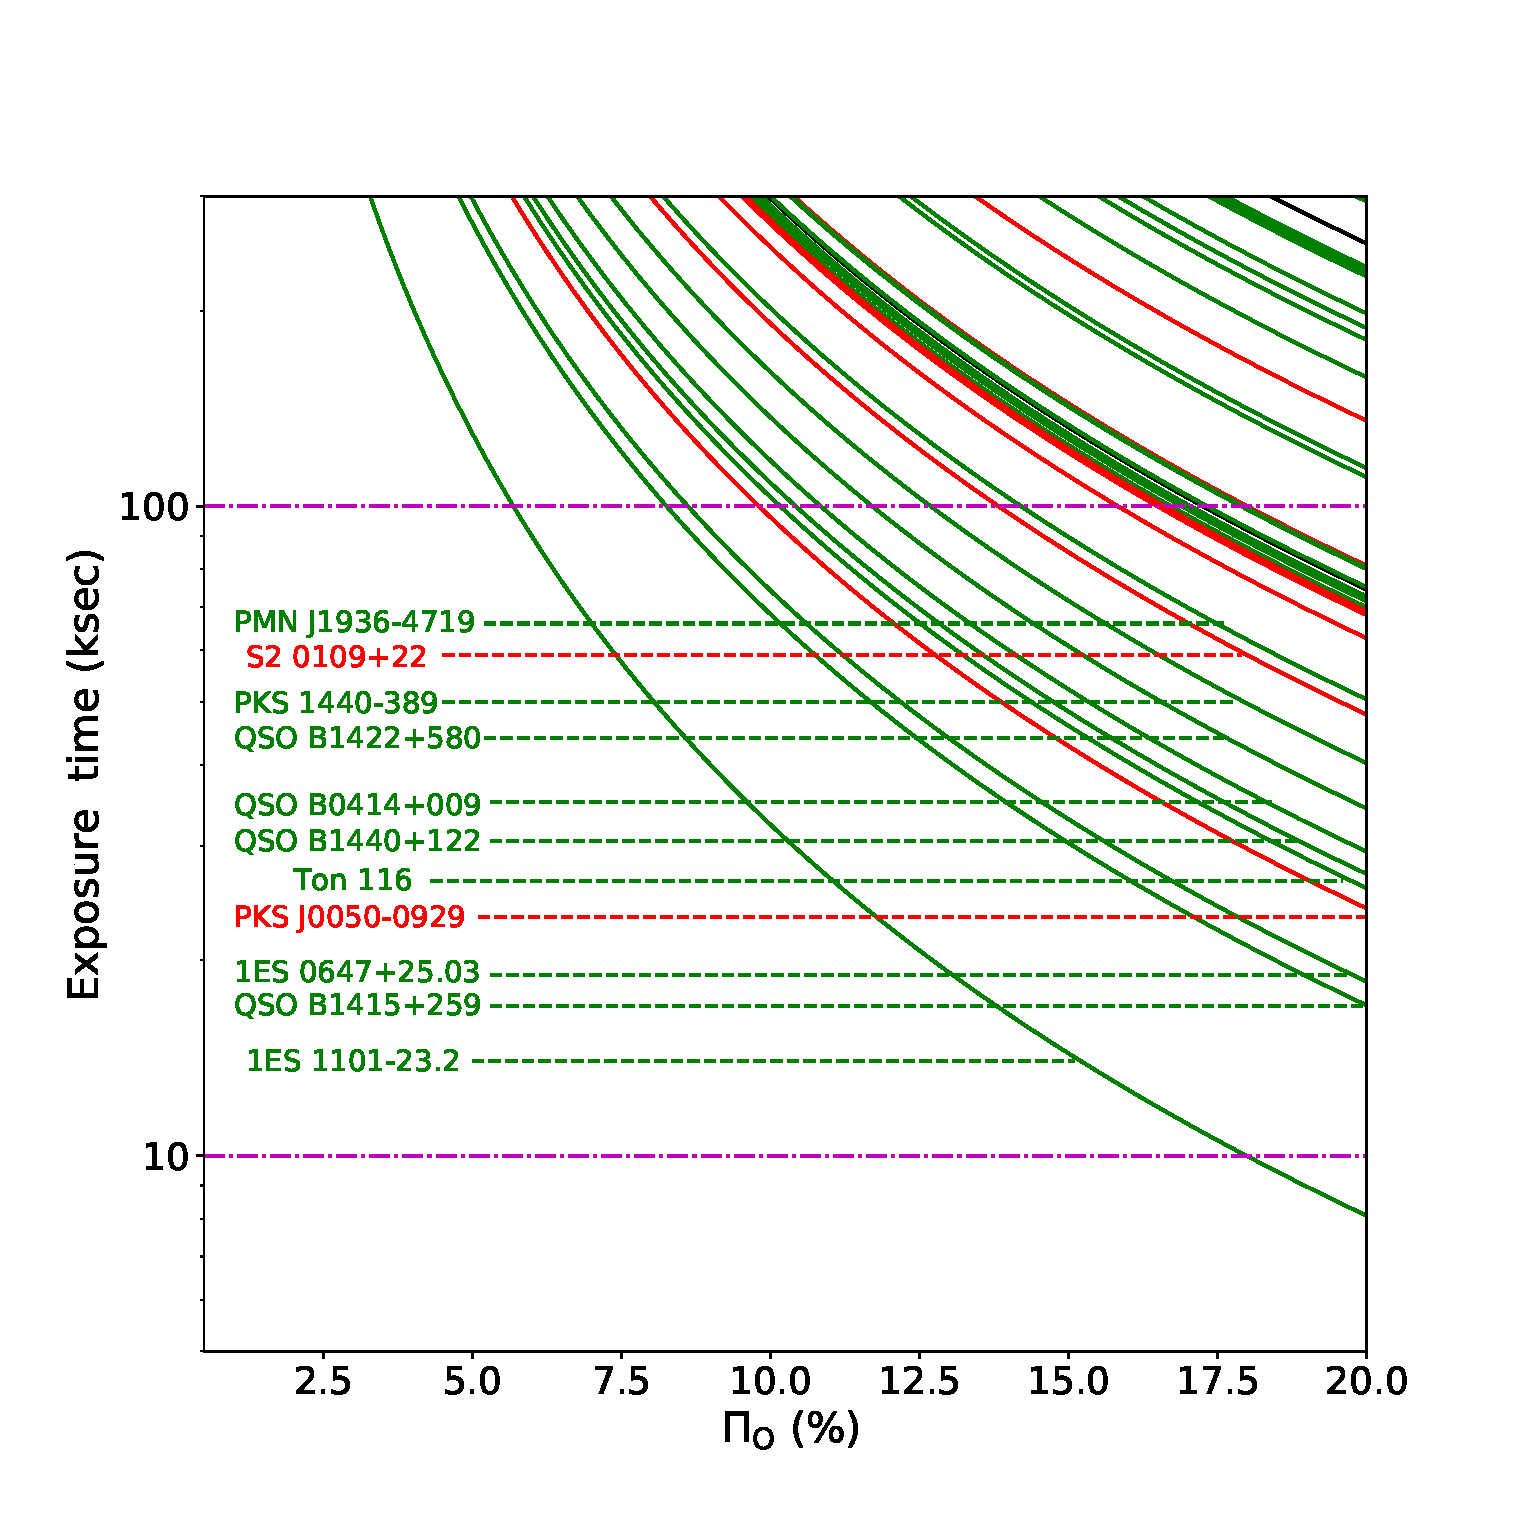
\includegraphics[scale=1]{exp_vs_pol.eps}}
\centering
\caption{Required {\it IXPE} exposure time as a function of (presently unknown) optical polarization level.
This $\rm \Pi_O$ has been corrected to an expected $\rm \Pi_X$, using the sources SEDs. The best prospects are
labeled. The sources are colored according to their SEDs: LSPs (black), ISPs (red) and HSPs (green).}
\label{fig:nopol}
\end{figure}


\subsection{Summary}
\label{sec:sum}

We have used the archival SEDs of bright blazars along with observed optical
polarization levels, to predict the expected 1-10\,keV X-ray polarization in a basic 
synchro-self Compton model. This estimate, together with the historical X-ray flux level
lets us evaluate the detectability of X-ray polarization for a given mission sensitivity.
Including the flux and polarization variability as estimated by cumulative distribution
functions modeled from historical data, lets us assess the probability that an exposure of given duration will achieve success. Equivalently, this gives the duty cycle for observations triggered by a monitoring campaign to be successful at a given exposure level. We compute these
values for the characteristic {\it IXPE} mission sensitivity, giving a list of top candidate 
sources, useful for planning an observing campaign. 

Unsurprisingly, HSP dominate the easily detectable sources, but a few ISPs with X-ray emission well above the synchrotron peak are surprisingly observable. In contrast few LSP can be accessed, and then only with long exposures. Recalling that our LSP estimate assumes correlated $\rm S_X/\Pi_O$ variability, and that no external seed photon flux dominates the up-scatter to the X-ray band, these LSP predictions  should be considered optimistic for a Synchro-Compton model. However, other emission scenarios (e.g. proton synchrotron) for the high energy component can produce large $\rm \Pi_X$, so a few LSP observations, especially when hadronic emission is indicated, would be desirable.

While our evaluation includes many of the brightest blazars, we have also identified a set which may be interesting targets, if the typical polarization level is sufficiently large. Optical reconnaissance to measure these $\rm \Pi_O$ and evaluate as possible targets for {\it IXPE} and/or {\it eXTP} are strongly encouraged.

\begin{table}
\caption{X-ray flux modeling results. The X-ray fluxes are all in $\rm erg/cm^2/s$ (log).}
\scriptsize
\begin{tabular}{lccccccc}
\toprule
Name & Alt. name & SED  & f & $\rm S_q$  & $\rm \sigma_q$ & $\rm S_a$  & $\rm \sigma_a$ \\
\midrule
J0152+0147 & 1RXS J015240.2+01 & HSP & - & -11.19 & 0.11 & - & - \\ 
J0210-5101 & PKS 0208-512 & LSP & 0.91 & -11.76 & 0.12 & -11.27 & 0.08  \\
J0222+4302 & 3C 66A & HSP & - & -11.16 & 0.06 & - & - \\ 
J0232+2017 & 1ES 0229+200 & HSP & 0.17 & -10.89 & 0.08 & -10.64 & 0.08  \\
J0238+1636 & PKS 0235+164 & LSP & 0.47 & -11.84 & 0.09 & -11.46 & 0.27 \\
J0324+3410 & 1H 0323+342 & HSP & - & -10.85 & 0.14 & - & - \\ 
J0530+1331 & PKS 0528+134 & LSP & - & -11.44 & 0.24 & - & - \\ 
J0539-2839 & PKS 0537-286 & LSP & - & -11.39 & 0.11 & - & - \\
J0559-5026 & PKS 0558-504 & - & - & -10.79 & 0.14 & - & - \\
J0721+7120 & S5 0716+714 & ISP & 0.16 & -11.1 & 0.35 & -10.21 & 0.15  \\
J0831+0429 & PKS 0829+046 & LSP & - & -11.46 & 0.08 & - & - \\
J0830+2410 & QSO B0827+243 & LSP & 0.79 & -11.70 & 0.13 & -11.08 & 0.12  \\
J0841+7053 & 4C 71.07 & LSP & - & -10.82 & 0.09 & - & - \\
J0854+2006 & OJ 287 & LSP & - & -11.37 & 0.18 & - & - \\
J1103-2329 & 1ES 1101-232 & HSP & 0.2 & -10.57 & 0.06 & -10.25 & 0.02  \\
J1104+3812 & Mrk 421 & HSP & 0.44 & -9.52 & 0.46 & -8.94 & 0.28  \\
J1159+2914 & 4C 29.45 & LSP & 0.23 & -11.46 & 0.09 & -11.08 & 0.03  \\
J1221+2813 & W Com & ISP & 0.73 & -12.07 & 0.06 & -11.80 & 0.22  \\
J1229+0203 & 3C 273 & LSP & 0.09 & -9.9 & 0.13 & -9.89 & 0.02  \\
J1256-0547 & 3C 279 & LSP & 0.83 & -11.24 & 0.09 & -10.94 & 0.21  \\
J1408-0752 & 1Jy 1406-076 & LSP & - & -12.25 & 0.09 & - & - \\ 
J1428+4240 & 1H 1430+423 & HSP & 0.52 & -10.64 & 0.2 & -10.08 & 0.12  \\
J1512-0905 & PKS 1510-089 & LSP & - & -11.07 & 0.13 & - & - \\ 
J1555+1111 & PG 1553+113 & HSP & 0.41 & -10.89 & 0.04 & -10.65 & 0.07  \\
J1626-2951 & PKS 1622-297 & LSP & 0.55 & -11.52 & 0.14 & -10.96 & 0.11  \\
J1635+3808 & 1Jy 1633+38 & LSP & - & -11.46 & 0.24 & - & -  \\
J1653+3945 & Mrk 501 & HSP & - & -9.66 & 0.24 & - & - \\ 
J1733-1304 & NRAO 530 & LSP & - & -11.45 & 0.11 & - & - \\
J1959+6508 & 1ES 1959+650 & HSP & 0.79 & -9.93 & 0.22 & -9.27 & 0.25  \\
J2009-4849 & PKS 2005-489 & HSP & 0.51 & -11.01 & 0.09 & -10.03 & 0.35  \\
J2158-3013 & PKS 2155-304 & HSP & 0.61 & -10.62 & 0.25 & -9.94 & 0.25  \\
J2202+4216 & BL Lacertae & LSP & 0.1 & -10.91 & 0.16 & -10.33 & 0.15  \\
J2232+1143 & CTA 102 & LSP & - & -11.02 & 0.08 & - & - \\
J2253+1608 & 3C 454.3 & LSP & 0.93 & -10.69 & 0.1 & -10.01 & 0.22  \\
J2347+5142 & 1ES 2344+514 & HSP & - & -10.47 & 0.23 & - & -  \\  
\bottomrule
\end{tabular}
\label{tab:par_sources}
\end{table}



\begin{table}
\caption{X-ray flux and polarization. The X-ray fluxes are all in $\rm erg/cm^2/s$ (log). Polarization degree is in \%. The table lists sources with $>0.5\%$ X-ray polarization and X-ray flux $\rm >5\times10^{-13} erg/cm^2/s$. The table lists only the first 10 sources. The table is published in its entirety in the machine-readable format. A portion is shown here for guidance regarding its form and content.}
\scriptsize
\begin{tabular}{lccccccccc}
\toprule
Name & Alt. name & Redshift & SED & $\rm \nu_{peak}$  & $\rm S$  & $\rm \sigma_S$ & $\rm \Pi_O$ & $\rm \sigma_{\Pi_O}$  & $\rm \Pi_X$ \\
\midrule
J0017-0512 & CGRaBSJ0017-0512 & 0.227 & LSP & 13.69 & -11.66 & 0.01 & 7.99 & 3.66 & 2.68  \\ 
J0035+5950 & 1ES0033+595 & 0.086 & HSP & 17.12 & -10.5 & 0.26 & 3.1 & 0.01 & 3.3  \\
J0045+2127 & RXJ00453+2127 & -- & HSP & 16.0 & -10.52 & 0.0 & 7.4 & 2.13 & 8.43  \\ 
J0102+5824 & PLCKERC217G124.4 & 0.664 & LSP & 12.94 & -11.52 & 0.06 & 15.9 & 8.27 & 5.14  \\
J0108+0135 & PKS0106+01 & 2.099 & LSP & 13.18 & -11.81 & 0.25 & 12.47 & 4.6 & 4.09  \\ 
J0136+4751 & S40133+47 & 0.859 & LSP & 13.08 & -11.59 & 0.02 & 11.5 & 5.76 & 3.75  \\ 
J0152+0146 & 1RXSJ015240.2+01 & 0.080 & HSP & 15.46 & -11.21 & 0.29 & 6.2 & 6.49 & 7.87  \\
J0211+1051 & CGRaBSJ0211+1051 & 0.200 & ISP & 14.12 & -11.33 & 0.41 & 23.1 & 6.93 & 35.0  \\
J0217+0837 & PLCKERC217G156.1 & 0.085 & LSP & 13.79 & -11.44 & 0.19 & 5.8 & 3.09 & 1.96  \\
J0222+4302 & 3C 66A & 0.340 & HSP & 15.09 & -11.16 & 0.36 & 7.8 & 2.94 & 11.1  \\
\bottomrule
\end{tabular}
\label{tab:xpol_pred}
\end{table}




\begin{table}
\caption{Detectability duty cycle. The table is sorted according to detection probability and lists only sources with DP$>1\%$.}
\scriptsize
\begin{tabular}{lcccc}
\toprule
Name & Alt. name  & SED & $\rm \nu_{peak}$ & Det. Prob. (\%) \\
\midrule
J1959+6508 & 1ES 1959+650 & HSP & 16.86 & 72.9 \\
J1725+1152 & 1H 1720+117 & HSP & 16.01 & 60.6 \\
J2001+4352 & 1FGL J2001.1+435 & HSP & 15.21 & 60.3 \\
J1104+3812 & Mrk 421 & HSP & 17.07 & 58.5 \\
J0211+1051 & CGRaBs J0211+1051 & ISP & 14.12 & 49.2 \\
J2158-3013 & PKS 2155-304 & HSP & 15.97 & 42.1 \\
J1653+3945 & Mrk 501 & HSP & 16.12 & 30.7 \\
J0222+4302 & 3C 66A & HSP & 15.09 & 17.0 \\
J1555+1111 & PG 1553+113 & HSP & 15.47 & 14.4 \\
J2253+1608 & 3C 454.3 & LSP & 13.34 & 10.2 \\
J0721+7120 & S5 0716+714 & ISP & 14.6 & 5.6 \\
J1838+4802 & GB6J1838+4802 & HSP & 15.8 & 4.5 \\
J2347+5142 & 1ES 2344+514 & HSP & 15.87 & 3.4 \\
J0958+6533 & S4 0954+658 & LSP & 13.49 & 3.4 \\
J2202+4216 & BL Lac & LSP & 13.61 & 2.5 \\
J1642+3948 & 3C 345 & LSP & 13.23 & 1.8 \\
J1256-0547 & 3C 279 & LSP & 13.11 & 1.8 \\
J0957+5522 & 4C 55.17 & ISP  & 14.23 & 1.5\\
\bottomrule
\end{tabular}
\label{tab:duty_cycle}
\end{table}



\begin{table}{lccccccc}
\caption{Sources without optical polarization. The X-ray fluxes are all in $\rm erg/cm^2/s$ (log). Column $\rm \Pi_{O,min}$ lists the minimum optical polarization degree (\%) required for an {\it IXPE} detection at 100ksec.}
\scriptsize
\begin{tabular}{lccccccc}
\toprule
Name & Alt. name & Redshift & SED & $\rm \nu_{peak}$  & $\rm S$  & $\rm \sigma_S$ & $\rm \Pi_{O,min}$ \\
\midrule
J0050-0929 & PKS J0050-0929 & 0.635 & ISP & 14.61 & -11.09 & 0.01 & 9.76  \\ 
J0112+2244 & S2 0109+22 & 0.265 & ISP & 14.32 & -11.62 & 0.02 & 13.76  \\ 
J0416+0105 & QSO B0414+009 & 0.287 & HSP & 16.64 & -10.7 & 0.02 & 10.79  \\ 
J0650+2502 & 1ES 0647+250 & 0.203 & HSP & 16.42 & -10.51 & 0.01 & 8.57  \\ 
J1103-2329 & 1ES 1101-23.2  & 0.186 & HSP & 17.19 & -10.07 & 0.01 & 5.66  \\ 
J1243+3627 & Ton 116 & 1.066 & HSP & 16.15 & -10.67 & 0.02 & 10.12  \\ 
J1417+2543 & QSO B1415+259 & 0.236 & HSP & 15.45 & -10.6 & 0.01 & 8.22  \\ 
J1422+5801 & QSO B1422+580 & 0.635 & HSP & 17.72 & -10.73 & 0.03 & 11.65  \\ 
J1442+1200 & QSO B1440+122 & 0.163 & HSP & 16.35 & -10.68 & 0.02 & 10.38  \\ 
J1443-3908 & PKS 1440-389 & 0.065 & HSP & 15.68 & -10.93 & 0.01 & 12.63  \\ 
J1936-4719 & PMN J1936-4719 & 0.265 & HSP & 16.52 & -10.94 & 0.03 & 14.14  \\  
\bottomrule
\end{tabular}
\label{tab:no_pol}
\end{table}



\section{Detecting X-ray polarization in ISP blazars}

Both leptonic and hadronic emission processes may contribute to blazar jet emission; which dominates in blazars's high energy emission component remains an open question. Some intermediate synchrotron peaked blazars transition from their low to high energy emission components in the X-ray band making them excellent laboratories to probe both components simultaneously, and good targets for the newly launched Imaging X-ray Polarimetry Explorer. We characterize the spectral energy distributions for three such blazars: CGRaBS~J0211+1051, TXS~0506+056, and S5~0716+714, predicting their X-ray polarization behavior by fitting a multizone polarized leptonic jet model. We find that a significant detection of electron synchrotron dominated polarization is possible with a 300~ks observation for S5~0716+714 and CGRaBS~J0211+1051 in their flaring states, while even 500~ks observations are unlikely to measure synchrotron self-Compton polarization. Importantly, non-leptonic emission processes like proton synchrotron are marginally detectable for our brightest ISP, S5~0716+714, during a flaring state. Improved {\it IXPE} data reduction methods or next generation telescopes like {\it eXTP} are needed to confidently measure SSC polarization.

Blazars are often classified by the peak frequency ($\nu_{Sy}$) of the low-energy component \citep{abdo_spectral_2010}. Here we focus on the ``Intermediate Synchrotron Peak'' (ISP) blazars, whose synchrotron emission  peaks in optical/UV and have their spectral energy distributions (SEDs) dropping toward eventual high-energy component dominance in the hard X-ray/$\gamma$-ray band. In particular, we focus on a subclass of ISPs whose X-ray emission lies in the valley formed by the combination of the two spectral components.

While the origin of the high-energy component is still unknown, the recent launch of the Imaging X-ray Polarimetry Explorer ({\it IXPE}, \citealp{weisskopf_imaging_2022}) offers a new diagnostic tool to probe the jet physics, composition, and acceleration of particles. In \citet{liodakis_prospects_2019} we used a multizone jet model \citep{marscher_turbulent_2014,peirson_polarization_2018,peirson_polarization_2019} and optical polarization results from the RoboPol survey \citep{blinov_robopol_2021} to make predictions for the X-ray polarization degree of blazars.  In a synchrotron self-Compton (SSC) scenario, we expect substantial polarization from the electron synchrotron and much lower polarization levels from the Compton component. On the other hand, the polarization degree of proton-synchrotron and synchrotron from hadron initiated pair cascades is expected to be much higher than that of IC emission and comparable to that of the primary electron synchrotron component. Interestingly, as one observes further out on the electron synchrotron cut-off tail, fewer jet emission zones have sufficient particle energies and Doppler factors to produce the detected radiation -- this means that there is decreased polarization angle (PA) averaging between emission zones and thus larger net synchrotron polarization degree and higher variability \citep{peirson_polarization_2018,peirson_polarization_2019}. Polarization measurements in the transition region between low- and high-energy components can thus be a powerful tool to probe not only for the high-energy emission processes, but also the jet and magnetic field structure. Coincidentally, recent hybrid (also known as lepto-hadronic) blazar models for the high-energy neutrino emission suggest the existence of subdominant synchrotron components from proton initiated pair cascades that might only be detectable in the transition valley where any primary lepton emission is minimized \cite[e.g.,][]{gao_modelling_2019}. All of the above suggest that ISPs, whose transition regions lie in the  1-10\,keV band are particularly attractive targets for current and future X-ray polarization missions.

We have identified three such sources, namely CGRaBS~J0211+1051, TXS~0506+056, and S5~0716+714. CGRaBS J0211+1051 and S5~0716+714 are first year {\it IXPE} targets, while  CGRaBS J0211+1051 and TXS 0506+056 are potential neutrino emitters \citep{icecube_multi-messenger_2018,hovatta_association_2021}. Our goal is twofold: (1) understand the polarization behaviour of the jet across the transition region; (2) make predictions for {\it IXPE} and future missions to understand the high-energy emission signatures from blazars. In \S\ref{sec:dm} we describe the data and jet models, in \S\ref{sec:ixpe} we make predictions for {\it IXPE}, and in \S\ref{sec:disc} we discuss our findings.

\subsection{Multiwavelength observations and modeling} 
\label{sec:dm}

The non-X-ray multiwavelength data for all sources are taken from the Space Science data center archive\footnote{\url{https://tools.ssdc.asi.it/SED/}}. The data are not contemporaneous and include both flaring and quiescent periods of each source. Since the latter may allow improved polarization measurements, we analyze quiescent and flaring data separately. We bin the observations in frequency bins of 0.1 dex and treat the resulting SED as an ``average'' SED of the source in the given state. Examples are shown in Fig.~\ref{fig:sed}.

For the X-ray observations we used publicly available Neil Gehrels Swift Observatory ({\it Swift}), {\it NuSTAR} and XMM-Newton data from the High Energy Astrophysics Science Archive Research Center (HEASARC) browse interface. The X-ray observations for the source in normal and flaring (f) states are drawn from the following date ranges: 
CGRaBS J0211+1051(f) (MJD 55260-55886),
CGRaBS J0211+1051 (MJD 59250),
S5~0716+714(f) (MJD 57046),
S5~0716+714 (MJD 54864-55920),
TXS 0506+056(f) (MJD 58025).
For CGRaBS J0211+1051 in quiescence we augment with a new $\sim65$~ks XMM-Newton observation (AO-19, ID number: 0861840101, MJD 59250). All {\it Swift} data used were contemporaneous (within 1-2 days) of exposures from one of the other facilities.  The data were processed using the standard HEASARC tools and recommended analyses.

Previous fits to these data have typically used absorbed broken powerlaw models for TXS~0506+056 \citep{icecube_multi-messenger_2018} and S5 0716+714 \citep{wierzcholska_first_2016}. Instead, we fit the extracted spectra, using {\it XSPEC}, with a more physically motivated model: the sum of two powerlaw components, subject to absorption by a Galactic neutral hydrogen column $\rm N_H$. For CGRaBS J0211+1051, the publicly available {\it Swift} snapshots did not provide sufficient signal-to-noise to unambiguously determine the shape of the 1-10~keV spectrum. We thus tried three models, a single power-law, a power-law with an exponential cut-off, and a sum of two power-laws. We then used the Akaike information criterion to select the model that best describes the data. Again the sum of two power-laws is preferred. The best-fit model parameters are given in Table \ref{tab:xspec}. 

\begin{table}[t]
\caption{X-ray spectral parameters. The $\rm \rm N_H$ values are given in units of $\times10^{22}~cm^{-2}$.}
\centering
\begin{tabular}{lccc}
    \toprule
     Name &  $\rm N_H$ &  $\Gamma_2$  &  $\Gamma_1$ \\
    \midrule
    CGRaBS~J0211+1051 & 0.16 & 1.18$\pm0.19$  & 2.68$\pm$0.4 \\
    TXS~0506+056 & 0.25 & 1.83$\pm$0.2 & 3.88$\pm$1.0 \\
    S5~0716+714 & 0.031 & 1.56$\pm0.33$ & 2.36$\pm$0.14 \\
    \bottomrule
\end{tabular}
\label{tab:xspec}
\end{table}

\subsubsection{SED modeling}
Our joint SED and polarization modeling uses the polarized leptonic jet emission model developed in \citet{peirson_polarization_2018,peirson_polarization_2019}, inspired partly by \citet{potter_synchrotron_2012, marscher_turbulent_2014}. It assumes an initial power-law electron population propagating along a relativistic conical jet. The jet cross section is divided into multiple magnetic field zones, with isotropically distributed field orientations. These magnetic fields are comoving with the jet material.

Polarized synchrotron emission is self-consistently calculated as the electron population propagates and cools. SSC emission is computed, including the propagation of synchrotron photons from downstream emission into each Comptonizing zone. For quasi-spherical magnetic field zones, as often assumed in turbulent scenarios, the model resolves a decorrelation timescale (which depends on the initial jet parameters) of 0.5--5 days. This is the timescale over which steady state jet emission is expected to fluctuate.

An important feature of this jet model is variable Doppler boosting of the zones, since those directed closest to the line of sight increasingly dominant in the observed flux as the SED steepens \citep{peirson_polarization_2019}. This guarantees an increasing expected polarization degree and larger polarization variability above the synchrotron peak. The X-ray SSC polarization degree is typically $\sim 0.2-0.35\times$ that of the synchrotron peak polarization; the components' PAs are highly correlated. In this model the observed synchrotron and SSC polarization behavior depends significantly on the geometric jet parameters, such as jet opening angle, observation angle, and Lorentz factor.

Our leptonic jet emission model is essentially independent of particle acceleration method since it follows zones downstream of any acceleration region. The assumed `chaotic' disordered magnetic fields and relativistic boosting effects should be present in many magnetic reconnection and shock acceleration scenarios. We also assume steady-state emission, probing polarization variability by re-seeding the magnetic field zones. We briefly discuss how these simplifying assumptions may be violated in other models found in the literature in \S\ref{sec:disc}.

\begin{figure}
\centering
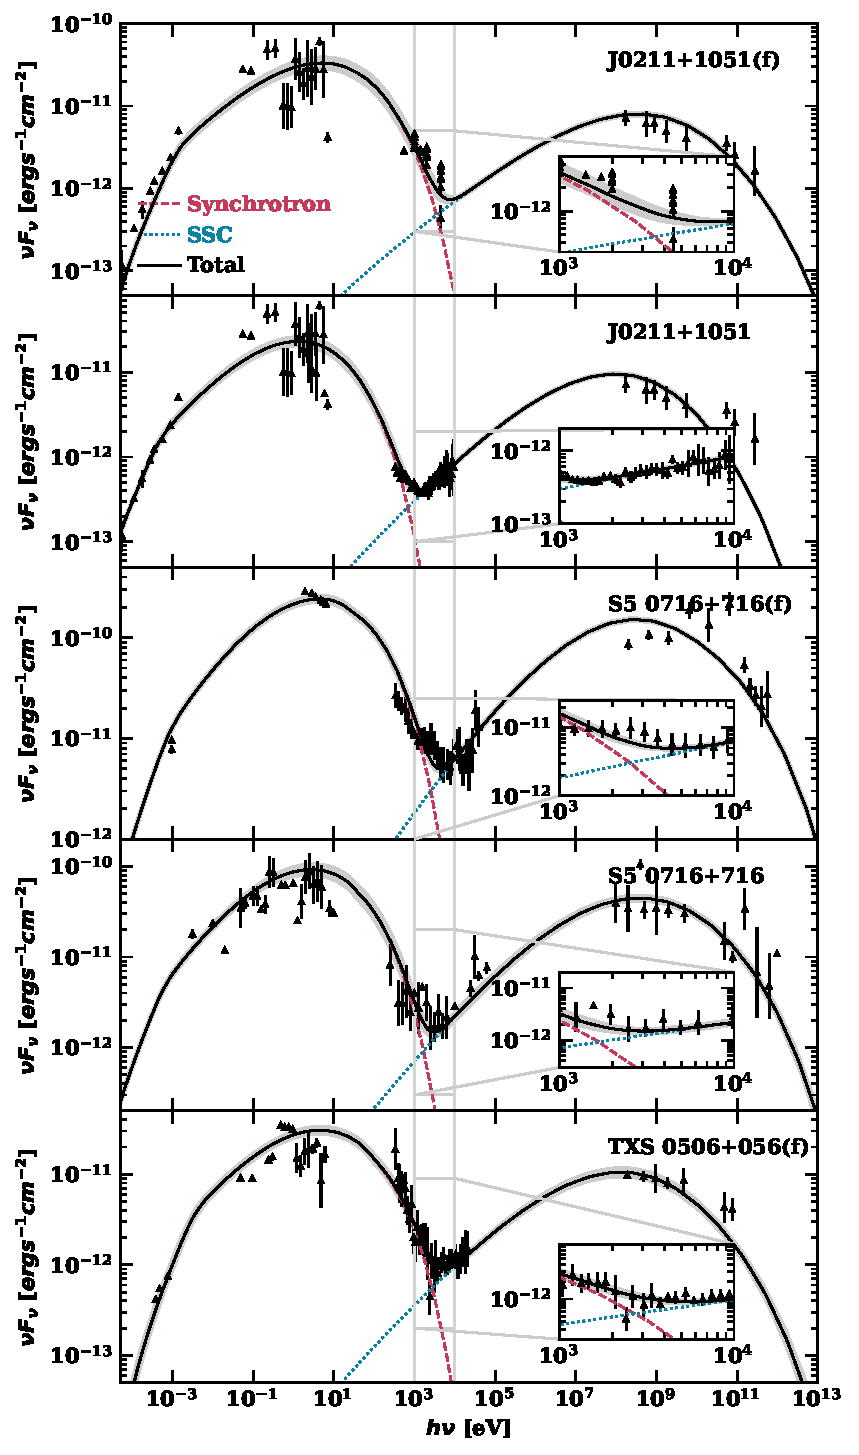
\includegraphics[width=0.5\textwidth]{figures/SED_all.pdf}
\caption{Polarized leptonic jet model fits to all blazars and states. `(f)' denotes a flaring state. Black traces show the expected total SED for the best fit jet parameters. Grey shaded regions around the black trace show $1\sigma$ model deviations due to different random magnetic field zones. Vertical grey lines denote {\it IXPE}'s sensitive band, $1-10$~keV, and insets show close-ups of this region.}
\label{fig:sed}
\end{figure}

In order to constrain our model's jet parameters, we fit the multiwavelength SED observations of each blazar state. Due to the chaotic magnetic field zones, our model is stochastic: the same jet parameters can result in different observed SEDs. A stochastic optimization method is necessary to fit such a model to fixed observations. We use a simple variant of the cross-entropy method \citep{rubinstein_cross_2004,kochenderfer_algorithms_2019}. At each step, this samples $n$ sets of jet parameters from a multivariate Gaussian and re-fits a new Gaussian using $k$ samples with the lowest $\chi^2$. Steps are repeated until convergence, when the mean and covariance matrix of the Gaussian no longer change significantly between steps. We use $n=80, k=20$. Since the multiwavelength SEDs for each blazar are not simultaneous and the true SEDs can be much more variable than the observational errors imply, we make the simplifying assumption that every observation has the same error. Our jet model has 8 free parameters. We open source the code to run our model and reproduce the results\footnote{\texttt{https://github.com/alpv95/SSCpol}} \citep{peirson_alpv95sscpol_2022}.

Model fit results are shown in Fig.~\ref{fig:sed}. Best fit jet parameters and their respective errors are displayed in Table~\ref{tab:jet}. In Fig.~\ref{fig:pol} we show the predicted polarization behavior resulting from the jet model fits displayed in Fig.~\ref{fig:sed}. The number of magnetic field zones in the jet model is selected so that the predicted optical polarization fraction matches the median of the observations \citep{blinov_robopol_2021} as closely as possible. Note that individual realizations of the polarization fraction can vary significantly.

\begin{table}[t]
\caption{Polarized jet model best fit parameters. Jet power $W_j$, electron high energy cutoff before exponential decay $E_{\rm max}$, electron population power law index $\alpha$, full conical jet opening angle in lab frame $\theta_{\rm open}$, bulk Lorentz factor $\Gamma_{\rm bulk}$, initial magnetic field strength $B_0$, jet observation angle in lab frame $\theta_{\rm obs}$, and initial equipartition fraction $A_{\rm eq}$. (f) denotes a flaring state. The number of magnetic field zones $N_{\rm zones}$ is selected from $[1,7,19,37,64,128]$. All blazar models shown here use 37 magnetic field zones except CGRaBS J0211+1051, which uses 19.}
\centering
\scriptsize
\begin{tabular}{lccccccccc}
    \toprule
    Name & $W_j [10^{37}W]$ &  {$E_{\rm max} [10^{9} eV]$} &  {$\alpha$}  &  {$\theta_{\rm open} [^\circ]$} &  {$\Gamma_{\rm bulk}$} &  {$B_0 [10^{-5}T]$} &  {$\theta_{\rm obs} [^\circ]$}  &  {$A_{\rm eq}$} \\
    \midrule
    J0211+1051(f) & $4.94 \pm 0.1$ & $13.4 \pm 1.0$ & $2.05 \pm 0.01 $ & $7.16 \pm 0.19$ & $14.8\pm 0.64$ & $5.04 \pm 0.2$ & $1.95\pm 0.18$ & $0.81\pm 0.01$\\
    J0211+1051 & $6.48 \pm 0.2$ & $9.59 \pm 0.1$ & $1.85 \pm 0.01 $ & $14.1 \pm 0.35$ & $7.23\pm 0.15$ & $2.38 \pm 0.2$ & $2.31\pm 0.09$ & $0.83\pm 0.02$\\
    TXS~0506+056 & $5.26 \pm 0.5$ & $8.03 \pm 0.3$ & $1.89 \pm 0.01 $ & $4.15 \pm 0.26$ & $17.3\pm 0.42$ & $9.63 \pm 0.3$ & $1.64\pm 0.11$ & $0.98\pm 0.05$\\
    S5~0716+714(f) & $42.4 \pm 5.0$ & $13.4 \pm 3.0$ & $1.66 \pm 0.02 $ & $7.35 \pm 0.62$ & $13.2\pm 0.51$ & $2.84 \pm 0.6$ & $2.51\pm 0.06$ & $1.05\pm 0.02$\\
    S5~0716+714 & $47.3 \pm 11.0$ & $9.49 \pm 1.5$ & $1.75 \pm 0.09 $ & $5.93 \pm 0.84$ & $17.0\pm 0.64$ & $3.23 \pm 1.5$ & $4.48\pm 0.16$ & $0.84\pm 0.13$\\
    \bottomrule
\end{tabular}
\label{tab:jet}
\end{table}

It is useful to compare our polarization predictions to previous studies. \citet{zhang_probing_2019} model TXS 0506+056 using a single zone leptonic emission model with a uniform magnetic field, matching the observed optical polarization degree with a constant polarization dilution factor. They predict an SSC polarization degree of approximately $5\%$ in the X-ray band, rising to $8\%$ at MeV energies. This represents a slightly higher X-ray polariztion fraction, increasing more strongly to high energy. The differences can be attributed to our multizone setup, where multiple magnetic field orientations relative to the line of sight affect the net synchrotron to SSC polarization ratio and its energy dependence \citep{bonometto_polarization_1973, peirson_polarization_2019}; multi-zone models generally predict lower SSC polarization degree. We note that our model also propagates synchrotron seed photons between magnetic field zones, further diluting the SSC polarization and increasing sensitivity to the jet geometry.

\begin{figure}
    \centering
    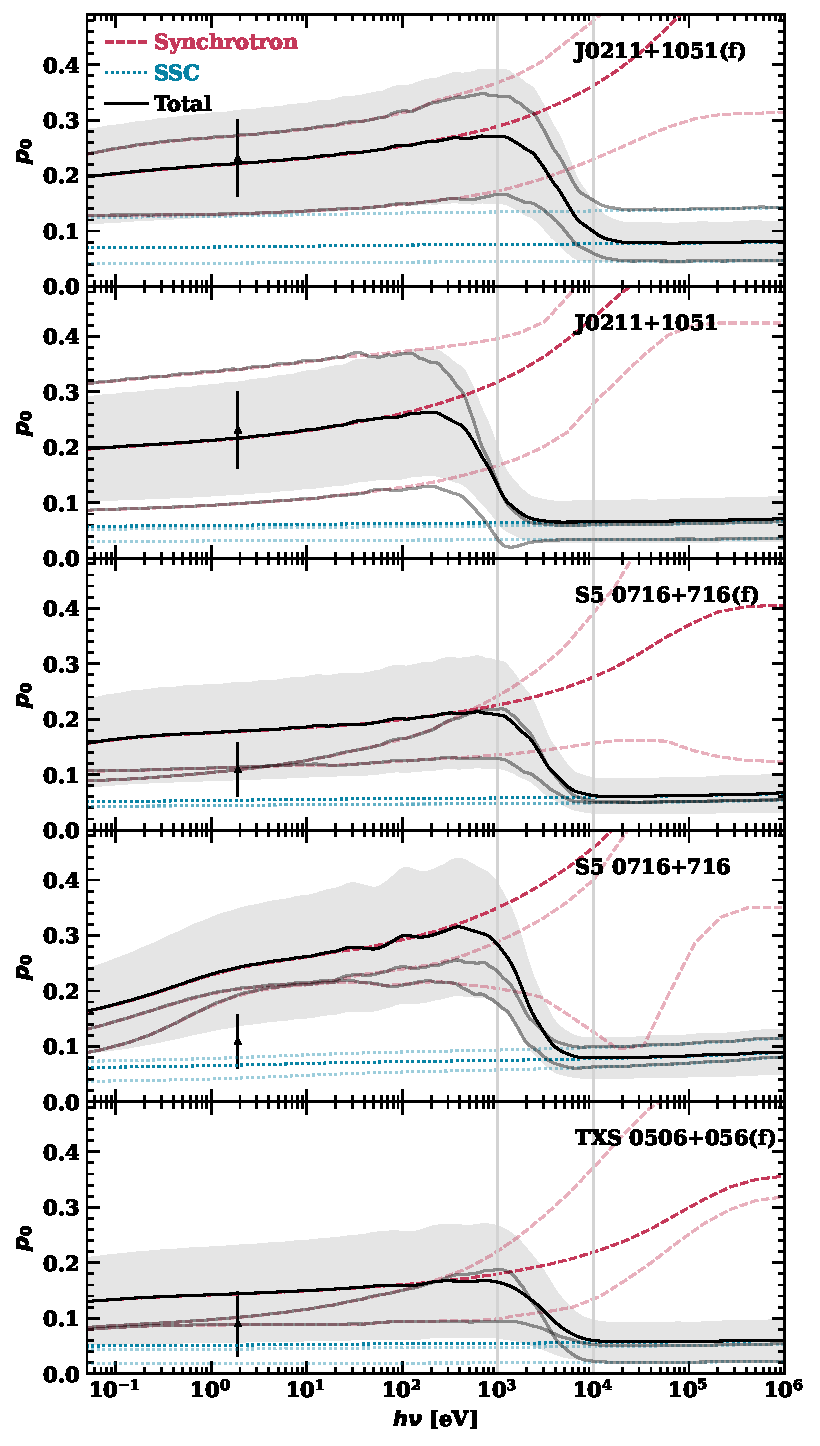
\includegraphics[width=0.5\textwidth]{figures/pol_all.pdf}
    \caption{Leptonic (SSC) jet model polarization fraction predictions. The jet models used in each panel are the same as those in Fig.~\ref{fig:sed}. Black observations denote the average measured optical polarization over multiple epochs (MJD 56432 -- 57893 for Robopol measured S5~0716+714 and J0211+1051 \citep{blinov_robopol_2021} and MJD 58019 -- 58267 for TXS~0506+056). Lines and shaded regions mean the same as Fig.~\ref{fig:sed} with the addition of two transparent models, which represent randomly selected model realizations.}
    \label{fig:pol}
\end{figure}

\subsection{{\it IXPE} Measurement Simulations}
\label{sec:ixpe}

A principal goal of {\it IXPE}-ISP source measurements is to detect two different X-ray polarizations -- a lower energy, electron synchrotron dominated component and a higher energy component.  Assuming an SSC spectrum, we explore whether such a measurement is possible for each of our ISPs with typical {\it IXPE} exposures, using {\it IXPE}'s standard analysis pipeline processing over a 2-8~keV band.  

Using \textit{ixpeobssim}, {\it IXPE}'s observation simulation software \citep{pesce-rollins_observation-simulation_2019}, we simulate multiple 300\,ks and 500\,ks observations for each blazar state assuming polarization and flux are fixed to their expected (average) values (i.e. the black traces in Figs.~\ref{fig:sed}, \ref{fig:pol}). We split the simulated 2-8\,keV data into two energy bins: 2-4\,keV and 4-8\,keV, extracting the polarization fractions by estimating the Stokes' parameters as in \citet{kislat_analyzing_2015}. Figure~\ref{fig:meas} summarizes the results.

In Fig.~\ref{fig:meas}, energy bins where the true polarization fraction distribution (blue, right-hand-side) is fully below the minimum detectable polarization (MDP$_{99}$) threshold (dotted lines) cannot produce significant ($\gtrsim 3\sigma$) detection of non-zero polarization in the given exposure time. MDP$_{99}$ is the 99th percentile upper confidence bound on polarization fraction for an unpolarized source. Energy bins with some or all of the true polarization distribution above MDP$_{99}$ can have significant detections, if their actual polarization is in the upper portion of the predicted range -- the measurement errors would be approximately given by the measured polarization fraction distributions for the most probable $p_0$ (red, left-hand-side). Planned observation times for first-year {\it IXPE} ISP targets, including CGRaBS~J0211+1051 and S5~0716+714, are expected to range from 200\,ks -- 400\,ks.  

For each blazar and state the two energy bins, 2-4\,keV and 4-8\,keV, contain different relative synchrotron and SSC contributions. Insets in Fig.~\ref{fig:sed} give the relative contributions. In non-flaring states, both energy bins are almost entirely dominated by SSC emission so measurement of the synchrotron cutoff component will not be possible.

Low significance polarization fraction measurements, below MDP$_{99}$, are strongly biased away from $p_0 = 0$. Strict non-negativity of $p_0$ forces measurement posteriors (red, Fig.~\ref{fig:meas}) to be asymmetric and for $\mathbb{E}(\hat{p}_0) > p_0$ (see, esp. CGRaBS~J0211+1051 quiescent panel). This highlights the danger of making polarization inferences using low significance point estimates. The measurement bias can be corrected using appropriate $p_0$ estimators \citep{simmons_point_1985}. 

\begin{figure}
    \centering
    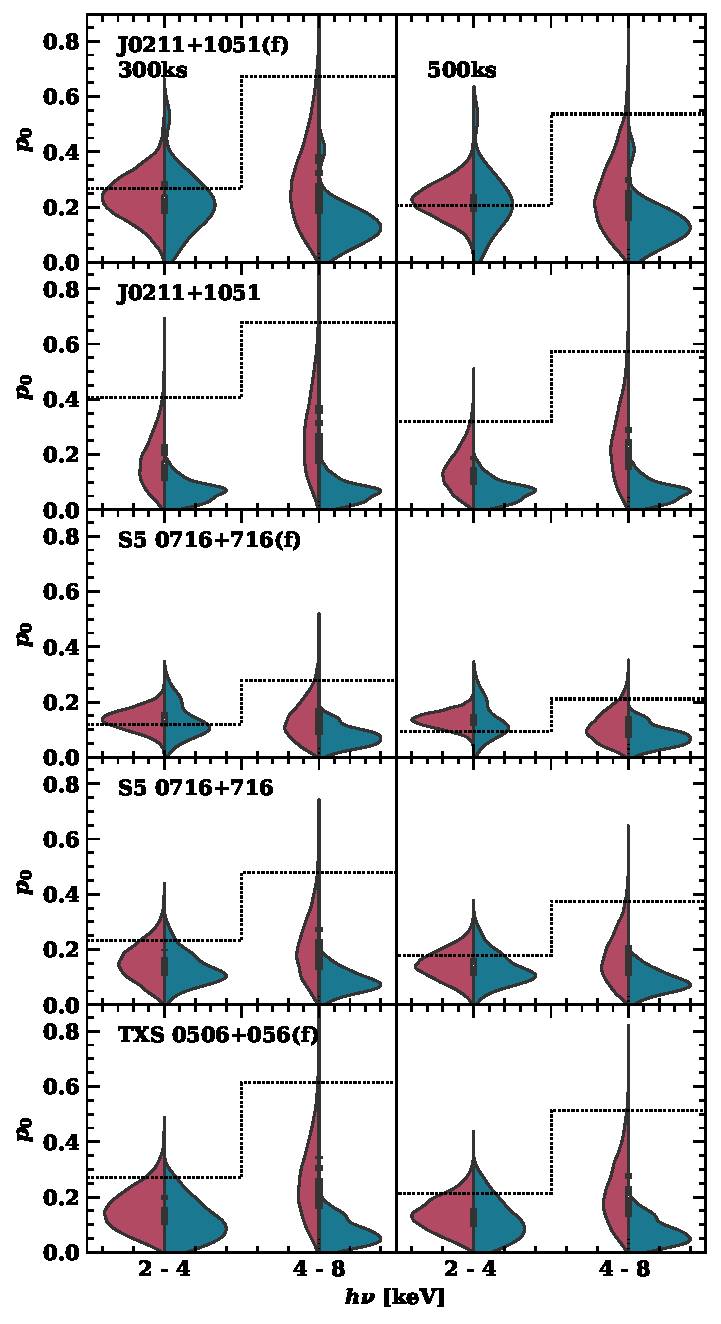
\includegraphics[width=0.5\textwidth]{figures/violin.pdf}
    \caption{Violin plots of the true polarization fraction distribution (blue, left-hand-side) and the measured polarization fraction distribution (red, right-hand-side) for $2-4$\,keV and $4-8$\,keV energy bins, and 300\,ks/500\,ks exposures. The distributions of true polarization fractions are extracted from our jet model fits (Fig.~\ref{fig:pol}) and are the same for both exposure times. Measured polarization fraction distributions assume a single observation with true polarization equal to the expected value.
    Dashed black traces represent the minimum detectable polarization (MDP$_{99}$) for each measurement bin. }
    \label{fig:meas}
\end{figure}

\subsection{Discussion} 
\label{sec:disc}
Under a purely leptonic (SSC) jet model for ISPs, we find that simultaneously detecting significant X-ray polarization from both emission components with a $\leq500$\,ks {\it IXPE} observation is impossible, even considering high $p_0$ fluctuations (see Fig.\ref{fig:meas}). 
For the assumptions used here, a $2.5$\,Ms exposure would be required to measure the median predicted SSC polarization in our brightest source, S5~0716+714, during its high state.
Unfortunately, blazar polarization variability may preclude such long observation times. Optical polarization measurements \citep{blinov_robopol_2021} suggest that blazar polarization fraction and PA can vary significantly over time periods $<500$\,ks. This would result in an incoherent averaging of polarization vectors leading to depolarization. Many blazar models \citep{marscher_turbulent_2014} including our own (Fig.~\ref{fig:pol}) predict polarized X-ray electron synchrotron emission to be more variable than the optical \citep{di_gesu_testing_2022}.

If external Compton (EC) contributes significantly to a blazar's high energy emission component, the case for measuring its X-ray polarization becomes even more dim. EC emission is usually assumed to be unpolarized \citep{zhang_x-ray_2013} since the external photon field being scattered is assumed incoherent, originating in the broad line region or accretion disk. Even a small EC contribution can make observations more difficult because MDP$_{99} \propto 1/\sqrt{N_{\rm ph}}$. A $10\%$ fractional EC contribution would lower Fig.~\ref{fig:meas} true polarization fractions by $10\%$ and increase required observation times for the same significance by $23\%$. 
Luckily, all three sources considered are classified as BL-Lac objects, typically associated with low EC contributions. \citet{padovani_txs_2019}, however, suggest that TXS 0506+056 is an FSRQ in disguise, in which case there might be significant EC contribution to the high energy component.

For the ISPs in flaring states, a significant polarization measurement of the synchrotron cutoff is feasible although still difficult, requiring the blazar to be in a high polarization state. Along the primary synchrotron cutoff we expect an increased expected polarization fraction and variability compared to the optical SED peak (see Fig.~\ref{fig:pol}) as the most Doppler-boosted magnetic field zones increasingly dominate the observed emission \citep{peirson_polarization_2019}.
%acceleration methods
Our model presents the minimal (geometry-induced) increase polarization degree above the primary synchrotron peak; other effects may further increase the dominance of individual zones.
For example, in the shock scenario particles are more efficiently accelerated when the magnetic field is aligned along the shock normal \citep{marscher_turbulent_2014}. Thus chaotic magnetic field zones will vary in their upper electron energy cutoff and that energy can correlate with the global jet geometry. The highest energy electrons contributing X-ray emission are close to the shock, where cooling is limited and the field orientation (and hence polarization) are more highly correlated. Also, \citet{tavecchio_probing_2018} show that immediately downstream of a shock magnetic field compression increases the field perpendicular to the shock normal; this preferential alignment tends to correlate the field orientations and increase net polarization degree, although such correlation decays as turbulence develops downstream. Both these effects may increase polarization at the high energy end of the synchrotron component, improving measurement prospects.  In contrast magnetic reconnection scenarios suggest synchrotron cutoff polarization with higher variability but similar net polarization degree to the synchrotron peak emission \citep{zhang_radiation_2020, tavecchio_probing_2018}. Thus comparing X-ray polarization to simultaneous optical polarization degree may be able to distinguish these acceleration scenarios. 

Unexpectedly large high energy component polarization arising from non-leptonic jet emission is possible and potentially detectable. Our leptonic (SSC) jet model predicts any high energy component polarization should typically be $0.2-0.35 \times$ lower than at the SED optical peak \citep{peirson_polarization_2019} with the decrement sensitive to the jet geometry. Of course, this ratio is variable and can occasionally fluctuate to large values $>0.5$, especially if the peak polarization is low, so only multi-epoch trends or long-term averages have predictive power.
In the most optimistic hadronic jet scenario, proton and secondary electron synchrotron dominate the high energy emission component \citep{zhang_x-ray_2013, gao_modelling_2019}. High energy component X-ray band polarization fractions would be similar to the SED optical peak (Fig.~\ref{fig:pol}), corresponding to a X-ray/optical polarization ratio of 1, extremely unlikely in a SSC dominant leptonic emission model. Although this would provide a much needed polarization fraction boost, a two component detection would remain out of reach, even for a $\leq500$\,ks {\it IXPE} observation, for all ISPs except S5~0716+714 in its flaring state. 
Indeed, S5~0716+714 is the first ISP {\it IXPE} target, planned for a 300\,ks observation on 31st March 2022; a significant polarization detection for both high and low energy components would be a promising indication of non-leptonic jet emission.

If initial {\it IXPE} observations do not detect significant polarization from either emission component in any ISPs, it will be difficult to rule out non-leptonic processes. Upper polarization fraction limits based on the MDP$_{99}$s in Fig.~\ref{fig:meas} will be too high to make any useful inference about the polarization ratio of the two emission components, even with a strong synchrotron detection at 2-4~keV. However, the measurements' sensitivity may be improved. Bayesian neural network analysis of {\it IXPE} data \citep{peirson_deep_2021, peirson_towards_2021} has been shown to reduce MDP$_{99}$s by up to $25\%$ compared to the standard {\it IXPE} analysis pipeline, as well as increasing {\it IXPE}'s effective energy band to 1-10\,keV. We may also tune the energy range of the `low' and `high' energy detection windows for an individual source's SED, improving our ability to measure or bound the two components' $p_0$. Such improved analysis could, for example, make a flaring 4-8~keV S5~0716+714 SSC polarization detection possible with a 500\,ks observation -- Fig.~\ref{fig:meas}. Although neural network analysis is not yet in production for {\it IXPE}, a re-analysis of borderline observations could reveal missed discoveries. Looking further ahead, the effective area of future X-ray polarization mission {\it eXTP} \citep{zhang_enhanced_2018} should be four times larger than {\it IXPE}'s, reducing MDP$_{99}$s by a factor of $0.5$ \citep{di_gesu_prospects_2020}. Including both improvements, simultaneous measurement of both ISP emission components with a 500~ks observation is well in scope for all the ISPs considered here.